\section{Code completion with NLMs}
Language modeling faces a complex problem when it comes to code completion. There are local (to only one block of code) and very long-distance dependencies in coding, such as initializing a variable only once per function. 
So, approaches like pointer networks(Ptr-Net)~\cite{pointer} were introduced, which involved merging a model employing pointer networks with attention, which was shown to perform better at simulating long-distance dependencies than traditional NLMs~\cite{ccnlm}.

By predicting words from the input sequence, Ptr-Nets offer a solution to the challenge of anticipating words that are not in one's vocabulary. However, Ptr-Nets can only expect words to appear in the local context because they cannot predict words outside the input sequence (like a block of code).
Due to this restriction, a mixture of Attention~(long dependencies) and Ptr-Nets~(local dependencies) called Pointer Mixture Network~\cite{ccnlm} was introduced. This model predicts words from the global vocabulary or copies one from a local context. 
In addition, a modified version of the Attention mechanism using an AST-based programming language was developed in this study~\cite{ccnlm}. These improvements to transformer architecture improved the performance of \cct{} and led to the creation of large language models like Codex~\cite{copilot}, which is the model used in the creation of Github Copilot~\cite{Copilot-web}.

% \subsection{Pointer Networks (Ptr-Net)}
% Pointer networks~\cite{pointer} are built on top of modified attention mechanism with pointers to input words. Figure~\ref{fig:1b} illustrates these pointers.

% \begin{figure}[hbt!]
% \centering 
% \subfloat[Sequence-to-Sequence.\label{fig:1a}]{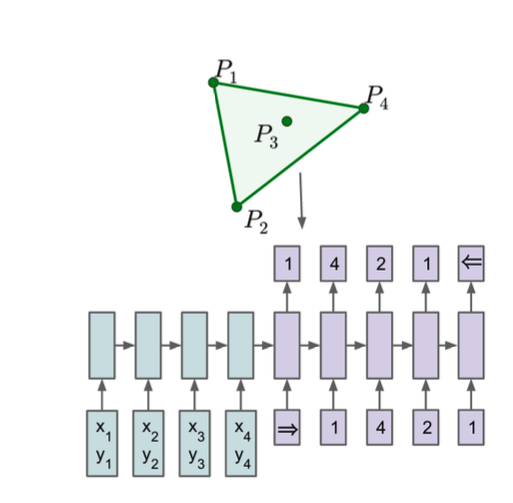
\includegraphics[width=0.5\textwidth]{Figures/seq.png}}\hfill
% \subfloat[Ptr-Net.\label{fig:1b}] {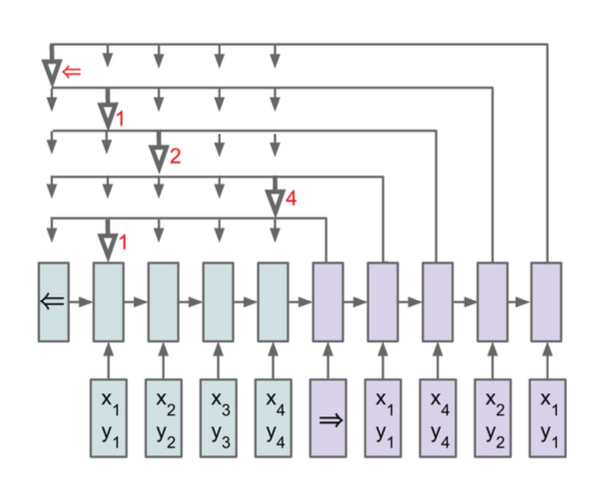
\includegraphics[width=0.5\textwidth]{Figures/soft_max.png}}
% \caption{Comparison of a Transformer (Sequence-to-Sequence model with a Ptr-Net.)~\cite{pointer}.} 
% \label{fig:pointer}
% \end{figure}

\subsection{GitHub Copilot}
Introduced in June 2021, GitHub's Copilot~\cite{Copilot-web} is an in-IDE recommender system that leverages OpenAI's Codex neural language model (NLM)~\cite{copilot} which uses a GPT-3 model~\cite{Gpt3}. This model comprises $\approx$13 billion parameters consuming hundreds of petaflop days to compute on Azure cloud platform~\cite{copilot} and is then fine-tuned on code from GitHub to generate code suggestions that are uncannily effective and can perform above human average on programming contest problems~\cite{empirical_eval}
While many other research projects have attempted to do something similar~\cite{codesearch, natural, coacor}, Copilot's availability and smooth integration with GitHub's backup have unavoidably generated a ``hype" in the tech community, with many developers either already using it through its technical preview or started using it after its recent public launch as a paid subscription~\cite{Copilot-web}. 

Using Copilot requires authorization using a GitHub account and is currently available for use on Visual Studio Code and other IDEs~\cite{Copilot-web}. GitHub Copilot provides suggestions for numerous languages and a wide variety of frameworks but works especially well for Python, JavaScript, TypeScript, Ruby, Go, C\# and C++~\cite{Copilot-web}. GitHub Copilot will automatically start giving suggestions when the user starts typing in the IDE, where the user has the option to use the suggestion, see alternative suggestions, or ignore the suggestion~\cite{Copilot-web}.

Currently, Copilot provides three key functionalities: autofill for repetitious code, suggest tests based on the implementation of code, and comment to code conversion~\cite{Copilot-web}. For the scope of this thesis, we focus on the feature of turning comments into code when a user adds a remark describing the logic they want to utilise~\cite{Copilot-web}. 
Although Copilot code suggestion can be triggered by adding a comment in natural language, it is advised that users add comments and meaningful names for function parameters to receive useful recommendations~\cite{Copilot-web}. 
The human input we used to trigger code suggestions from Copilot concatenates the natural language comment, function name, and function parameters.

Vaithilingam et al.~\cite{Vaithilingam2022} conducted an exploratory study of how developers use Copilot, finding that Copilot did not solve tasks more quickly but did save time in searching for solutions. 
More importantly, Copilot solved the writer's block problem of not knowing how to get started. This notion of seeding an initial, if incorrect, solution is often how design proceeds in software. 

Recent work shows initial investigations on how large language models for code can add architecture tactics by using program synthesis~\cite{Shokri2021, jigsaw} and structure learning~\cite{Karmakar2021}.
This thesis complements these earlier approaches by focusing on moving beyond code completion, where most research effort is currently concentrated.
To provide deeper insights into the overall effectiveness of the instrument, it is crucial to evaluate the quality of Copilot's suggestions and understand its limitations.

\subsection{Alternatives to Copilot}
There are a handful of code completion systems currently being used. Below is a list of few such systems:

\begin{itemize}
    \item Jedi~\cite{jedi} - An open source Python static analysis tool aimed at automatic code completion. Jedi has a focus on autocompletion and goto functionality. Other features include refactoring, code search, and finding references. However, performance issues and limitations on project size and complexity hamper its effectiveness.
    \item Kite~\cite{kite} - Kite is an AI-powered code completion plugin that works with 16 languages and 16 IDEs. It uses machine learning to rank completions more intelligently based on your current code context~\cite{kite}.
    \item Deep TabNine~\cite{tabnine} - Deep TabNine is a source code completion system which is based on OpenAI's GPT-2 Model~\cite{gpt2}. It is trained on GitHub public repositories with permissive open-source licenses. Trained code is also filtered to ensure quality and avoid outdated, esoteric, auto-generated code and other edge cases~\cite{tabnine}.
    \item AlphaCode~\cite{alphacode} - An \cct{} by DeepMind, which uses a transformer language model to generate code, pre-trained on selected GitHub code and fine-tuning on a curated set of competitive programming problems~\cite{alphacode}. The training process for AlphaCode included tests for code cloning, sensitivity to problem descriptions, and metadata. AlphaCode model focuses on creating novel solutions to problems that require deeper reasoning. 
    \item CodeBERT~\cite{codebert} - A bimodal pre-trained model for programming language (PL) and natural language (NL) by Microsoft. it uses multi-layer bidirectional Transformers for code completion~\cite{codebert}. CodeBERT learns general-purpose representations that support downstream NL-PL applications such as natural language code search, code documentation generation, etc. CodeBERT improved state-of-the-art performance on natural language code search and code documentation generation~\cite{codebert}.
    \item Amazon CodeWhisperer~\cite{amazon} - A machine learning powered service that helps improve developer productivity by generating code recommendations based on their comments in natural language and code. It supports Python, Java and JavaScript~\cite{amazon}. The code recommendations provided by CodeWhisperer are based on models trained on various data sources, including Amazon and open-source code~\cite{amazon}. CodeWhisperer also examines the code of the current file and other files in the developer's project to produce its recommendations~\cite{amazon}.
\end{itemize}
